\documentclass[11pt, oneside]{article} 
\usepackage{geometry}
\geometry{letterpaper} 
\usepackage{graphicx}
	
\usepackage{amssymb}
\usepackage{amsmath}
\usepackage{parskip}
\usepackage{color}
\usepackage{hyperref}

\graphicspath{{/Users/telliott/Github/figures/}}
% \begin{center} \includegraphics [scale=0.4] {gauss3.png} \end{center}

\title{Six functions}
\date{}

\begin{document}
\maketitle
\Large
\subsection*{basic definitions}
The most elementary trigonometric functions are the sine and cosine.  These are defined in  geometry as ratios of the lengths of the sides of a right triangle.  

Looking at the left panel, we say that the sine of the angle $\alpha$ is the ratio \emph{opposite-over-hypotenuse}, while the cosine of $\alpha$ is the ratio \emph{adjacent-over-hypotenuse}.  Tangent is the ratio \emph{opposite-over-adjacent}. The names are abbreviated to three letters in formulas.  

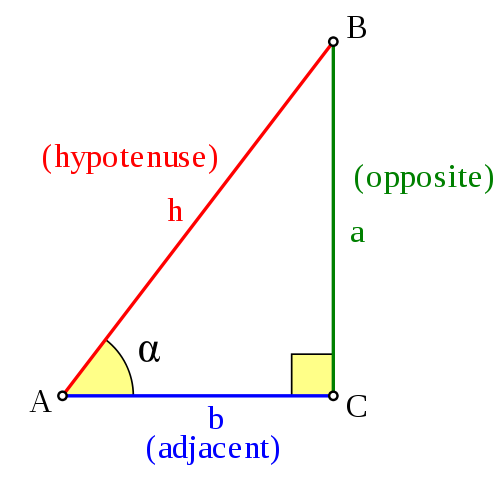
\includegraphics [scale=0.3] {sine_cosine.png}
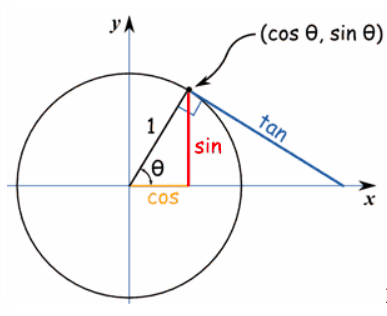
\includegraphics [scale=0.5] {sine_cosine_tangent.png}

Using the notation for the sides from the figure:
\[ \sin \alpha = \frac{a}{h}, \ \ \ \ \ \cos \alpha = \frac{b}{h}, \ \ \ \ \ \tan \alpha = \frac{a}{b} = \frac{\sin \alpha}{\cos \alpha} \]

The "unit circle" is a circle of radius $1$ with its center positioned at the origin of coordinates, the place where the $x$ and $y$ axes cross.  From the right panel of the diagram you can see that any point $(x,y)$ on the unit circle can be described in radial coordinates as 
\[ x = \cos \theta \ \ \ \ y = \sin \theta \]
In the diagram, all three right triangles are similar because the red line is an altitude of the largest right triangle.  Thus, by similar triangles, the blue side has this relationship
\[ \frac{\text{blue side}}{1} = \frac{\sin \theta}{\cos \theta} \]
which explains why it is labeled as $\tan$ ($\alpha$).

If the vertex labeled $B$ is denoted angle $\beta$ (the complementary angle of $\alpha$), then the notions of opposite and adjacent switch so that:
\[ \sin \alpha = \cos \beta, \ \ \ \ \ \cos \alpha = \sin \beta \]

If the circle has radius $r$ then
\[ x = r \cos \theta  \ \ \ \  y = r \sin \theta \]

Stewart:

\begin{quote}
The mathematicians of ancient India built on the Greek work to make major advances in trigonometry. They [used] the sine (sin) and cosine (cos) functions, which we still do today. Sines first appeared in the Surya Siddhanta, a series of Hindu astronomy texts from about the year 400, and were developed by Aryabhata in Aryabhatiya around 500. Similar ideas evolved independently in China.
\end{quote}

The other functions are the inverses of sine, cosine and tangent, namely:  cosecant, secant and cotangent.  The secant (inverse cosine) comes up somtimes, but the other two are not especially important in calculus.  

However, there is one context that we will look at, namely, Archimedes determination of the value of $\pi$.  The crucial step in that approach will turn out to be the calculation of the cotangent of the half-angle $\theta/2$ given the values of cotangent and cosecant for angle $\theta$.

The main relationship or identity is derived from the Pythagorean theorem.  We had above that for a unit circle
\[ x = r \cos \theta  \ \ \ \  y = r \sin \theta \]
Since $x$ and $y$ are the sides of a right triangle whose hypotenuse is $r$
\[ x^2 + y^2 = r^2 \]
and for a unit circle
\[ \cos^2 \theta + \sin^2 \theta = 1 \]
which is usually written
\[ \sin^2 \theta + \cos^2 \theta = 1 \]
and transformed to
\[ 1 + \tan^2 \theta = \sec^2 \theta \]

\subsection*{particular values}
We can easily determine the values for these functions for three special cases.  

The first is the angle $45$ degrees or $\pi/4$.  Draw an isosceles right triangle with sides of length $1$ (left panel).

\begin{center} 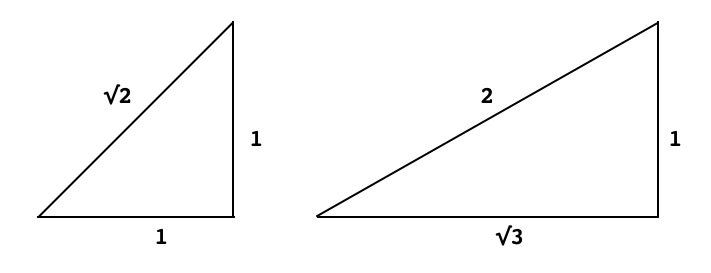
\includegraphics [scale=0.4] {30_45_60.png} \end{center}

Then the hypotenuse has length $\sqrt{2}$ (from Pythagoras) and the values are
\[ \sin \frac{\pi}{4} = \frac{1}{\sqrt{2}} = \cos \frac{\pi}{4} \]
\[ \tan \frac{\pi}{4} = 1 \]

For the other two, bisect an equilateral triangle and erase one half (right panel).  The smaller angle is $30$ degrees or $\pi/6$ and its complement is $60$ degrees or $\pi/3$.

The values are
\[ \sin \frac{\pi}{6} = \frac{1}{2} = \cos \frac{\pi}{3}, \ \ \ \ \ \ \cos \frac{\pi}{6} = \frac{\sqrt{3}}{2} = \sin \frac{\pi}{3} \]
\[ \tan \frac{\pi}{6} = \frac{1}{\sqrt{3}} \]

We can easily verify that 
\[ (\frac{1}{2})^2 + (\frac{\sqrt{3}}{2})^2 = 1, \ \ \ \ \ \  (\frac{1}{\sqrt{2}})^2 + (\frac{1}{\sqrt{2}})^2 = 1 \]

\subsection*{graph}

\begin{center} 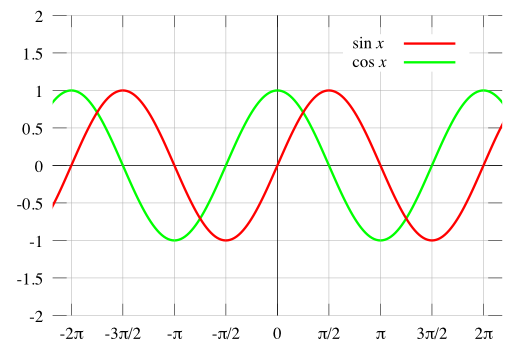
\includegraphics [scale=0.4] {sine_cosine_wikipedia.png} \end{center}

Savov:

\begin{quote}The sine function represents a fundamental unit of vibration. The graph of $\sin(x)$ oscillates up and down and crosses the $x$-axis multiple times. The shape of the graph of $\sin(x)$ corresponds to the shape of a vibrating string.\end{quote}

Imagine a circle placed to the left of a graph.  I think of the sine function as the "shadow" of the point ($x,y$) as it travels around the circle at the same constant speed as the point on the graph "moves" to the right.

\subsection*{visualization of all six functions}

Consider a unit circle.  Extend the radius with the angle $\theta$ and then draw the vertical and horizontal tangents to the circle $a$ and $b$.  

\begin{center} 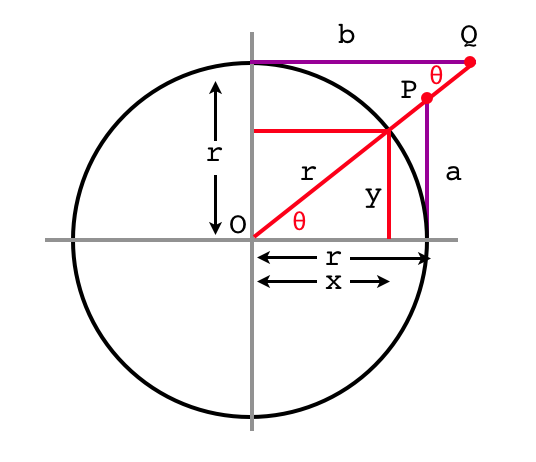
\includegraphics [scale=0.4] {sixfuncs1.png} \end{center}
The original triangle with sides $x,y,r$ is similar to the triangle with sides $r,a,OP$, and both are similar to the triangle with sides $b,r,OQ$.
\[ x,y,r \sim r,a,OP, \sim b,r,OQ \]
By similar $\triangle$
\[ \frac{a}{r} = \frac{y}{x} =  \tan \theta \]
But $r=1$ so 
\[ a = \tan \theta \]
If you imagine a point moving around the circle $a$ will get very large as $\theta \to \pi/2$, and in fact, approaches $\infty$ there (becomes undefined).

The segment $OP$ is (by similar $\triangle$) to $r$ as
\[ \frac{OP}{r} = \frac{r}{x} \]
\[ OP = \frac{1}{\cos \theta} = \sec \theta \]

The horizontal from the y-axis to Q is $b$.  Consider $\theta$ near the top of the figure.  By similar $\triangle$, the relations we had were
\[ r/b = y/x = \tan \theta  \]
since $r = 1$
\[ b = \frac{r}{\tan \theta} = \frac{1}{\tan \theta} = \cot \theta \]
Finally
\[ r/OQ = 1/OQ = \sin \theta \]
\[ OQ = \frac{1}{\sin \theta} = \csc \theta \]

\begin{center} 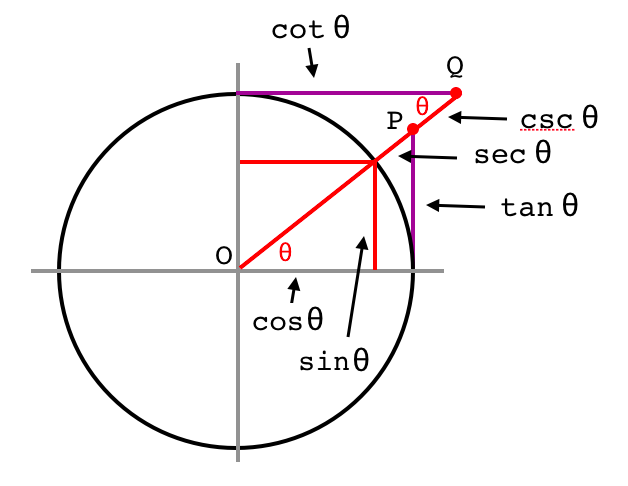
\includegraphics [scale=0.4] {sixfuncs3.png} \end{center}

\end{document}